\documentclass[a4paper,11pt]{ltjsarticle}

\usepackage[top=25mm,bottom=25mm,left=25mm,right=25mm]{geometry}
\usepackage{graphicx}
\usepackage{hyperref}

\title{第一回レポート}
\author{学籍番号: 2313188 \\ 藤田愛海}
\date{}

\begin{document}

\maketitle

\section{目的}
本課題では，事前学習済みAlexNetを用いて転送学習を行い，小型家電・周辺機器画像の分類性能を評価する。AlexNetは大規模画像データで学習済みの畳み込みニューラルネットワークであり，画像のエッジ，色，形状などの一般的な特徴表現をすでに獲得している。そのため，少量の画像データでも，最後の分類層を新しいタスクに合わせて調整することで分類モデルを構築できると考えられる。

\section{使用データ}
分類対象は，charger，earphone，mouse，power\_strip，remote の5クラスとした。各クラス21枚，合計105枚の画像を用意した。画像はカテゴリごとのフォルダに保存し，MATLABの imageDatastore を用いてフォルダ名を正解ラベルとして読み込んだ。

各クラスの画像枚数は以下の通りである。
\begin{itemize}
  \item charger: 21枚
  \item earphone: 21枚
  \item mouse: 21枚
  \item power\_strip: 21枚
  \item remote: 21枚
\end{itemize}

データは \path{splitEachLabel(imds, 0.7, "randomized")} により，各クラスごとに70\%を学習データ，30\%を検証データにランダム分割した。その結果，学習画像数は70枚，検証画像数は35枚となった。

\begin{figure}[htbp]
  \centering
  \begin{minipage}[t]{0.3\linewidth}
    \centering
    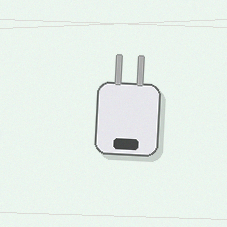
\includegraphics[width=\linewidth,height=30mm,keepaspectratio]{assets/sample_images/charger_01.png}
    \par\small charger
  \end{minipage}
  \hfill
  \begin{minipage}[t]{0.3\linewidth}
    \centering
    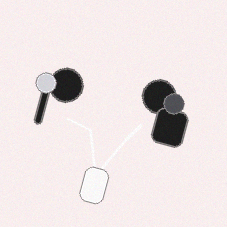
\includegraphics[width=\linewidth,height=30mm,keepaspectratio]{assets/sample_images/earphone_01.png}
    \par\small earphone
  \end{minipage}
  \hfill
  \begin{minipage}[t]{0.3\linewidth}
    \centering
    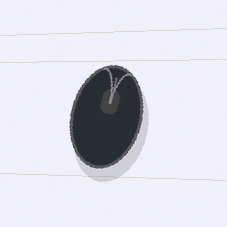
\includegraphics[width=\linewidth,height=30mm,keepaspectratio]{assets/sample_images/mouse_01.png}
    \par\small mouse
  \end{minipage}

  \vspace{2mm}

  \begin{minipage}[t]{0.3\linewidth}
    \centering
    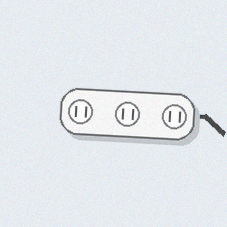
\includegraphics[width=\linewidth,height=30mm,keepaspectratio]{assets/sample_images/power_strip_01.png}
    \par\small power\_strip
  \end{minipage}
  \hfill
  \begin{minipage}[t]{0.3\linewidth}
    \centering
    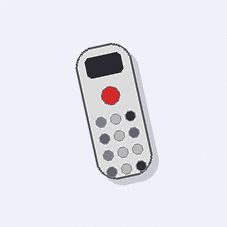
\includegraphics[width=\linewidth,height=30mm,keepaspectratio]{assets/sample_images/remote_01.png}
    \par\small remote
  \end{minipage}
  \hfill
  \begin{minipage}[t]{0.3\linewidth}
    \centering
    \vspace{18mm}
  \end{minipage}
  \caption{各カテゴリから1枚ずつ抽出したサンプル画像}
  \label{fig:sample-images}
\end{figure}

\section{方法}
事前学習済みAlexNetを読み込み，最終分類層を本実験のクラス数である5クラスに合わせて変更した。AlexNetの入力サイズは227$\times$227$\times$3であるため，\texttt{augmentedImageDatastore} を用いて入力画像を自動的に227$\times$227へリサイズした。

AlexNetは入力画像サイズが227$\times$227$\times$3に固定されているため，元画像のサイズが異なっていても，学習前にすべて227$\times$227ピクセルへ統一する必要がある。ここで3はRGBの3チャンネルを表す。227$\times$227は一見小さい入力サイズに見えるが，本実験の分類対象はマウス，イヤホン，電源タップ，リモコン，充電器のように形状の違いが比較的大きい物体であるため，分類に必要な特徴は十分保持されていたと考えられる。実際に，検証精度は約94.3\%となり，高い分類性能が得られた。

また，学習データに対してランダム左右反転および平行移動を用いたデータ拡張を行った。これにより，少ない画像枚数でも撮影角度や位置の違いに対してある程度頑健な学習を行うことを目的とした。

学習にはSGDMを用い，損失関数にはクロスエントロピーを使用した。学習条件は，MiniBatchSize=10，MaxEpochs=6，InitialLearnRate=1e-4 とした。

\section{発生した問題と対応}
学習時に，検証データが無効であるというエラーが発生した。原因は，データセット内にRGB画像とグレースケール画像が混在していたことである。AlexNetは入力として3チャンネルのRGB画像を必要とするため，1チャンネルのグレースケール画像が混ざると，\texttt{augmentedImageDatastore} の処理でエラーになる。

この問題に対して，\texttt{augmentedImageDatastore} のオプションに \path{ColorPreprocessing="gray2rgb"} を指定し，グレースケール画像をRGB画像に変換することでチャンネル数を3に統一した。

\section{結果}
学習は最大エポック数6/6で停止し，反復回数は42回であった。実行時間は約31秒であり，ハードウェアリソースは単一CPUであった。学習率は0.0001で一定とし，ValidationFrequency=3により3反復ごとに検証を行った。

\begin{figure}[htbp]
  \centering
  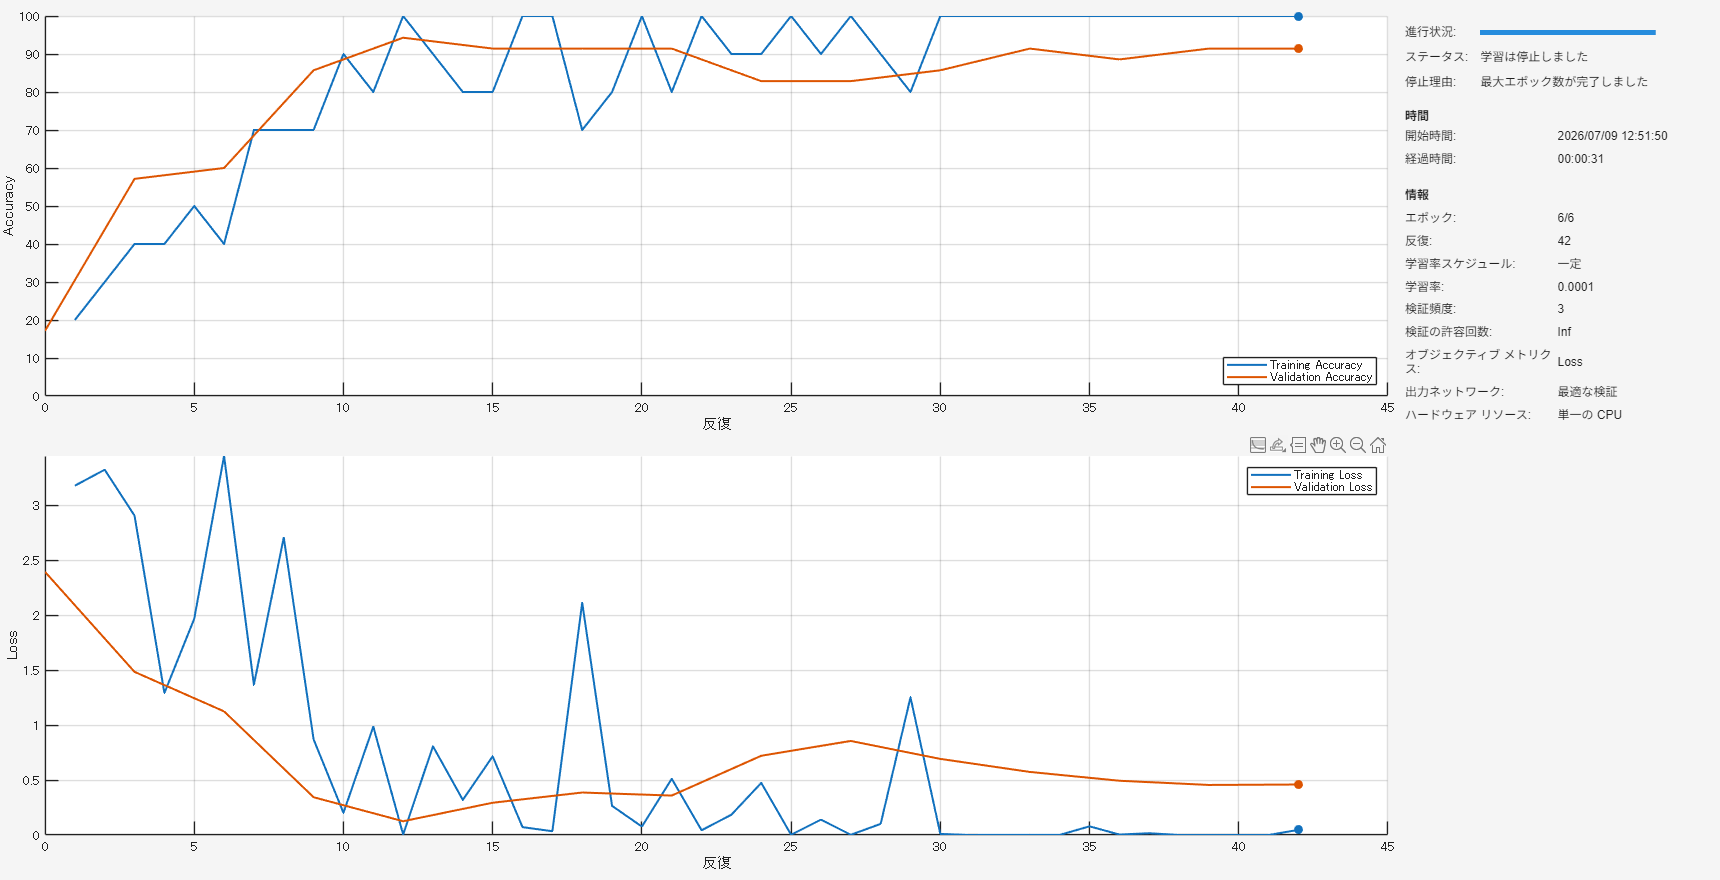
\includegraphics[width=\linewidth]{assets/alexnet_training_curve.png}
  \caption{AlexNetの転送学習における学習精度・検証精度および損失の推移}
  \label{fig:alexnet-training-curve}
\end{figure}

学習曲線を見ると，学習精度は反復が進むにつれて上昇し，最終的にほぼ100\%に到達した。検証精度も序盤から上昇し，10反復前後で90\%付近に達した。その後も大きく低下せず，おおむね90\%以上を維持した。

学習後，検証データ35枚に対して分類を行い，予測ラベルと正解ラベルを比較して分類精度を算出した。その結果，検証精度は0.94286，すなわち約94.3\%であった。これは35枚中33枚を正しく分類し，2枚を誤分類したことを意味する。

また，\texttt{confusionchart} により混同行列を表示し，どのカテゴリ間で誤分類が発生したかを確認した。特に，charger と power\_strip はどちらもコンセントやケーブルを含むため，形状が似ており誤分類が起こりやすいと考えられる。一方で，mouse や remote は形状が比較的特徴的であるため，分類しやすい可能性がある。

\section{考察}
転送学習では，AlexNetが事前学習によって獲得した一般的な画像特徴を利用できるため，少量の画像でも分類モデルを構築できる。本実験では各クラス21枚という比較的少ないデータ数であったが，最後の分類層を5クラス分類用に変更し，既存の特徴抽出能力を利用することで分類を行った。

誤分類が発生した場合，原因として以下が考えられる。第一に，charger と power\_strip のように物体の形状や色が似ているカテゴリでは，画像特徴が近くなりやすい。第二に，画像枚数が少ないため，モデルが物体そのものではなく背景や撮影条件を手がかりにしてしまう可能性がある。第三に，画像検索で収集した画像には構図や解像度のばらつきがあり，カテゴリ内の特徴が安定しにくい可能性がある。

\section{改善案}
分類精度が十分でない場合は，画像枚数を増やすことが最も有効である。特に誤分類が多いカテゴリの画像を追加することで，カテゴリ間の違いをより学習しやすくなる。また，回転や拡大縮小などのデータ拡張を追加することで，撮影条件の違いに対して頑健なモデルにできる可能性がある。さらに，MaxEpochsを増やして学習回数を調整することも改善策として考えられる。

\section{結論}
本実験では，事前学習済みAlexNetを用いて，小型家電・周辺機器画像の5クラス分類を行った。各クラス21枚，合計105枚という少量の画像データであったが，検証精度は約94.3\%となり，転送学習により高い分類性能が得られることを確認した。一方で，検証画像数は35枚と少ないため，この精度のみで汎化性能を断定することはできない。今後は，誤分類が多いカテゴリの画像追加，データ拡張の強化，学習回数の調整を行うことで，分類精度と評価の信頼性を向上できると考えられる。

\end{document}
